\documentclass[
	10pt,								% globale Schriftgröße
	parskip=half-,						% setzt Absatzabstand hoch
	paper=a4,							% Format
	english,ngerman,					% lädt Sprachpakete
	]{scrartcl}							% Dokumentenklasse

% //////////////////// Pakete laden ////////////////////
\usepackage{amsmath}			% MUSS vor fontspec geladen werden
\usepackage{mathtools}			% modifiziert amsmath
\usepackage{amssymb}			% mathematische symbole, für \ceckmarks
\usepackage{amsthm}				% für proof
\usepackage{mathrsfs}			% für \mathscr
\usepackage{latexsym}
\usepackage{marvosym}				% für Lightning

\usepackage{fontspec} 			% funktioniert nur mit den neueren Compilern z.B. XeLaTeX
\usepackage{microtype}			% für bessere Worttrennung
\usepackage[ngerman]{babel} 	% Spracheinstellung
\usepackage{lmodern}			% verändert verwendete Schriftart, damit sie weniger pixelig ist

\usepackage{verbatim}
\usepackage{listings}			% Für Quellcode

\usepackage{graphicx}
\usepackage{tabularx}			% für Tabellen mit gleicher Spaltenbreite und automatischen Umbrüchen
\usepackage{fullpage}
\usepackage{multirow}			% für multirow in tabulars
\usepackage{rotate}
\usepackage[cmyk,table]{xcolor} % um Farben zu benutzen, kann mehr als das Paket color
\usepackage[					% Verlinkungen
	colorlinks,					% farbige Schrift, statt farbiger Rahmen
	linktocpage,				% verlinkt im Abb.Verzeichnis Seitenzahl statt Bildunterschrift
	linkcolor=blue				% setzt Farbe der Links auf blau
	]{hyperref}					% nur für digitale Anwendungen, url = "http://www.example.com"
\usepackage{url}				% für Webadressen wie e-mail usw.: "\url{http://www.example.com}"

\usepackage{enumerate}			% für versch. Aufzählungezeichen wie z.B. a)
\usepackage{xspace}				% folgt ein Leerzeichen nach einem \Befehl, wird es nicht verschluckt.
\usepackage{cancel}				% für das Durchstreichen u.a. in Matheformeln mit \cancel
\usepackage{float}              % zum Forcieren der Position von figure-Umgebungen

% zum Zeichnen (u.a. von Graphen)
\usepackage{fp}
\usepackage{tikz}
\usetikzlibrary{tikzmark}			% für \tikzmark{toRemember}
\usetikzlibrary{positioning}	% verbesserte Positionierung der Knoten
\usetikzlibrary{automata}		% für Automaten (GTI)
\usetikzlibrary{arrows}
\usetikzlibrary{shapes}
\usetikzlibrary{decorations.pathmorphing}
\usetikzlibrary{decorations.pathreplacing}
\usetikzlibrary{decorations.shapes}
\usetikzlibrary{decorations.text}

% //////////////////// Syntaxhighlighting ////////////////////
\lstloadlanguages{Python, Haskell, [LaTeX]TeX, Java}
\lstset{
   basicstyle=\footnotesize\ttfamily,	% \scriptsize the size of the fonts that are used for the code
   backgroundcolor = \color{bgcolour},	% legt Farbe der Box fest
   breakatwhitespace=false,	% sets if automatic breaks should only happen at whitespace
   breaklines=true,			% sets automatic line breaking
   captionpos=t,				% sets the caption-position to bottom, t for top
   commentstyle=\color{codeblue}\ttfamily,% comment style
   frame=single,				% adds a frame around the code
   keepspaces=true,			% keeps spaces in text, useful for keeping indentation
							% of code (possibly needs columns=flexible)
   keywordstyle=\bfseries\ttfamily\color{codepurple},% keyword style
   numbers=left,				% where to put the line-numbers;
   							% possible values are (none, left, right)
   numberstyle=\tiny\color{codegreen},	% the style that is used for the line-numbers
   numbersep=5pt,			% how far the line-numbers are from the code
   stepnumber=1,				% nummeriert nur jede i-te Zeile
   showspaces=false,			% show spaces everywhere adding particular underscores;
							% it overrides 'showstringspaces'
   showstringspaces=false,	% underline spaces within strings only
   showtabs=false,			% show tabs within strings adding particular underscores
   flexiblecolumns=false,
   tabsize=1,				% the step between two line-numbers. If 1: each line will be numbered
   stringstyle=\color{orange}\ttfamily,	% string literal style
   numberblanklines=false,				% leere Zeilen werden nicht mitnummeriert
   xleftmargin=1.2em,					% Abstand zum linken Layoutrand
   xrightmargin=0.4em,					% Abstand zum rechten Layoutrand
   aboveskip=2ex, 
}

\lstdefinestyle{py}{
   language=Python,
}
\lstdefinestyle{hs}{
   language=Haskell,
}
\lstdefinestyle{tex}{
	language=[LaTeX]TeX,
	escapeinside={\%*}{*)},     % if you want to add LaTeX within your code
	texcsstyle=*\bfseries\color{blue},% hervorhebung der tex-Schlüsselwörter
	morekeywords={*,$,\{,\},\[,\],lstinputlisting,includegraphics,
	rowcolor,columncolor,listoffigures,lstlistoflistings,
	subsection,subsubsection,textcolor,tableofcontents,colorbox,
	fcolorbox,definecolor,cellcolor,url,linktocpage,subtitle,
	subject,maketitle,usetikzlibrary,node,path,addbibresource,
	printbibliography},% if you want to add more keywords to the set
     numbers=none,
     numbersep=0pt,
     xleftmargin=0.4em,
}

\lstdefinestyle{java}{
	language=Java,
	extendedchars=true,		% lets you use non-ASCII characters;
   						% for 8-bits encodings only, does not work with UTF-8
}

\lstdefinelanguage[x64]{Assembler}     % add a "x64" dialect of Assembler
   [x86masm]{Assembler} % based on the "x86masm" dialect
   % with these extra keywords:
   {morekeywords={CDQE,CQO,CMPSQ,CMPXCHG16B,JRCXZ,LODSQ,MOVSXD, %
                  POPFQ,PUSHFQ,SCASQ,STOSQ,IRETQ,RDTSCP,SWAPGS, %
                  rax,rdx,rcx,rbx,rsi,rdi,rsp,rbp, %
                  r8,r8d,r8w,r8b,r9,r9d,r9w,r9b}
}					% for 8-bits encodings only, does not work with UTF-8

\lstdefinestyle{c}{
	language=c,
	extendedchars=true,		% for 8-bits encodings only, does not work with UTF-8
}

% //////////////////// eigene Kommandos ////////////////////
\newcommand\FU{Freie Universität Berlin\xspace}% benötigt package xspace
\newcommand\gdw{g.\,d.\,w.\xspace}
\newcommand\oBdA{o.\,B.\,d.\,A.\xspace}
\newcommand{\Eu}{\texteuro}
\newcommand\N{\mathbb{N}\xspace}
\newcommand\Q{\mathbb{Q}\xspace}
\newcommand\R{\mathbb{R}\xspace}
\newcommand\Z{\mathbb{Z}\xspace}
\newcommand\ohneNull{\ensuremath{\backslash\lbrace 0\rbrace}}% \{0}
\let\dhALT\dh	% Schreibt Befehl \dh in \dhALT um
\renewcommand\dh{d.\,h.\xspace}	%renew überschreibt command \dh
\newcommand\Bolt{\;\text{\LARGE\raisebox{-0.3em}{\Lightning}\normalsize}\xspace}% Blitz
\newcommand\zz{\ensuremath{\raisebox{+0.25ex}{Z}% zu zeigen
			\kern-0.4em\raisebox{-0.25ex}{Z}%
			\;\xspace}}
\newcommand{\from}{\ensuremath{\colon}}
\newcommand{\floor}[1]{\lfloor{#1}\rfloor}
\newcommand{\ceil}[1]{\lceil{#1}\rceil}
 \renewcommand{\L}{\ensuremath{\mathcal{L}}\xspace}
 \renewcommand{\P}{\ensuremath{\mathcal{P}}\xspace}
 \newcommand{\NL}{\ensuremath{\mathcal{N}\kern-0.2em\mathcal{L}}\xspace}
 \newcommand{\NP}{\ensuremath{\mathcal{NP}}\xspace}

% //////////////////// Mathefunktionen ////////////////////
\DeclareMathOperator{\Landau}{\mathcal{O}}
\DeclareMathOperator{\True}{True}
\DeclareMathOperator{\False}{False}

% //////////////////// eigene Theoreme ////////////////////
\newtheorem{theorem}{Satz}
\newtheorem{corollary}[theorem]{Folgerung}
\newtheorem{lemma}[theorem]{Lemma}
\newtheorem{observation}[theorem]{Beobachtung}
\newtheorem{definition}[theorem]{Definition}
\newtheorem{Literatur}[theorem]{Literatur}
% konfiguriert proof
\makeatletter
\newenvironment{Proof}[1][\proofname]{\par
  \pushQED{\qed}%
  \normalfont \topsep6\p@\@plus6\p@\relax
  \trivlist
  \item[\hskip\labelsep
%         \itshape
        \bfseries
    #1\@addpunct{.}]\ignorespaces
}{%
  \popQED\endtrivlist\@endpefalse
}
\makeatother

% //////////////////// eigene Farben ////////////////////
\let\definecolor=\xdefinecolor
\definecolor{FUgreen}{RGB}{153,204,0}
\definecolor{FUblue}{RGB}{0,51,102}

\definecolor{middlegray}{rgb}{0.5,0.5,0.5}
\definecolor{lightgray}{rgb}{0.8,0.8,0.8}
\definecolor{orange}{rgb}{0.8,0.3,0.3}
\definecolor{azur}{rgb}{0,0.7,1}
\definecolor{yac}{rgb}{0.6,0.6,0.1}
\definecolor{Pink}{rgb}{1,0,0.6}

\definecolor{bgcolour}{rgb}{0.97,0.97,0.97}
\definecolor{codegreen}{rgb}{0,0.6,0}
\definecolor{codegray}{rgb}{0.35,0.35,0.35}
\definecolor{codepurple}{rgb}{0.58,0,0.82}
\definecolor{codeblue}{rgb}{0.4,0.5,1}

% //////////////////// eigene Settings ////////////////////

\textheight = 230mm		% Höhe des Satzspiegels / Layouts
\footskip = 10ex			% Abstand zw. Fußzeile und Grundlinie letzter Textzeile
\parindent 0pt			% verhindert Einrückung der 1. Zeile eines Absatzes
\setkomafont{sectioning}{\rmfamily\bfseries}% setzt Ü-Schriften in Serifen, {disposition}											% bindet Header ein (WICHTIG)
\usepackage{graphicx}
\usepackage{amsmath}
\usepackage{amssymb}

\newcommand{\dozent}{Prof. Dr. Margarita Esponda}					% <-- Names des Dozenten eintragen
\newcommand{\tutor}{Lilli Walter}						% <-- Name eurer Tutoriun eintragen
\newcommand{\tutoriumNo}{6}				% <-- Nummer im KVV nachschauen
\newcommand{\projectNo}{3}									% <-- Nummer des Übungszettels
\newcommand{\veranstaltung}{Nichtsequentielle Programmierung}	% <-- Name der Lehrveranstaltung eintragen
\newcommand{\semester}{SoeSe 2017}						% <-- z.B. SoSo 17, WiSe 17/18
\newcommand{\studenten}{Boyan Hristov, Sergelen Gongor}			% <-- Hier eure Namen eintragen
% /////////////////////// BEGIN DOKUMENT /////////////////////////


\begin{document}
% /////////////////////// BEGIN TITLEPAGE /////////////////////////
\begin{titlepage}
	\subject{\dozent}
	\title{\veranstaltung, \semester}
	\subtitle{\Large Project \projectNo\\ \large\vspace{1ex} TutorIn: \tutor\\ Tutorium \tutoriumNo}
	\author{\studenten}
	\date{\normalsize \today}
\end{titlepage}

\maketitle								% Erstellt das Titelblatt
\vspace*{-10cm}							% rückt Logo an den oberen Seitenrand
\makebox[\dimexpr\textwidth+1cm][r]{	%rechtsbündig und geht rechts 1cm über Layout hinaus
	
\includegraphics[width=0.4\textwidth]{src/fu_logo} % fügt FU-Logo ein
}
% /////////////////////// END TITLEPAGE /////////////////////////

\vspace{7cm}							% Abstand
\rule{\linewidth}{0.8pt}				% horizontale Linie										% erstellt die Titelseite


Link zum Git Repository: \url{https://github.com/BoyanH/FU-Berlin-ALP4/tree/master/Solutions/Homework3}

% /////////////////////// Aufgabe 1 /////////////////////////
\section{Aufgabe}

\begin{align}
	& \lozenge \square A \Leftrightarrow \square \lozenge A \\
	\Leftrightarrow & \exists j \geq i: \square A \text{ in } S_j \Leftrightarrow 
	\forall j' \geq i: \lozenge A \text{ in } S_{j`} \\
	\Rightarrow &  \forall j' \geq i: \lozenge A \text{ in } S_{j`} \Rightarrow 
	\exists j \geq i: \square A \text{ in } S_j \\
	\Leftrightarrow & \exists j \geq i: ( \lozenge A \Rightarrow \square A ) \text{ in } S_j
\end{align}

$3 \Leftrightarrow 4$: Aber da $\lozenge A$ in alle $j' \geq i$ gilt, dann auch in j! Widerspruch! 

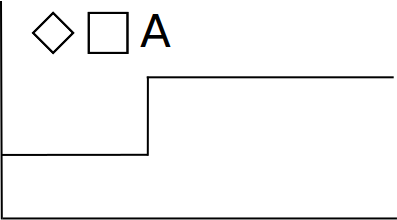
\includegraphics[width=\textwidth / 2]{./1_a.png}
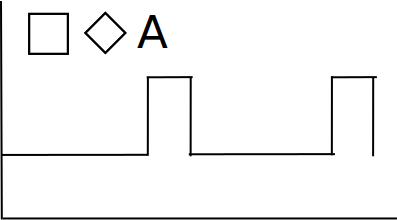
\includegraphics[width=\textwidth / 2 ]{./1_b.png}

\section{Aufgabe}

\begin{align}
	& \square A \Rightarrow \lozenge B \land \lozenge \square A \\
	\Leftrightarrow & \forall j \geq i A \text{ in } S_j \Rightarrow \exists k \geq i: B \text { in } S_k \land \exists l \geq i \forall p \geq l A \text{ in } S_p \\
	\Rightarrow & \exists l \geq i \exists k \geq l: B \text{ in } S_k \\
	\Leftrightarrow & \exists k \geq l: B \text{ in } S_k \\
	\Leftrightarrow & \lozenge B 
\end{align}

Informal: Wenn A immer gilt, dann gilt irgendwann B (Implikation) UND in irgendeinem Zustand $S_j, j \geq i$ gilt immer A. Dann wird ab $S_j$ die linke Seite der Implikation gelten, muss also die Rechte auch gelten.

\section{Aufgabe}

\begin{itemize}
	\item[a)]

	\begin{align}
		& ( \square A \land \square B) \Leftrightarrow \square (A \land B) \\
		\Leftrightarrow & \forall k \geq i: A \text{ in } S_k \land \forall l \geq i: B 
		\text{ in } S_l \\
		\Leftrightarrow & \forall k \geq i: A \text{ in } S_k \land \forall
		k \geq i: B \text{ in } S_k \\
		\Leftrightarrow & \forall k \geq i: A \land B \text{ in } S_k \\
		\Leftrightarrow & (A \land B)
	\end{align}

Informal: Die Distributivität ist hier anhand von triviale Umformungen mit Quantoren bewiesen. Wenn etwas für alle $k \geq i$ und für alle $l \geq i$ gilt, dann ist es egal welche von beiden wir nehmen, da beide von dem selben Wert (i) gelten und dann für ALLE Nachfolger. Wenn dann zwei mit logischem AND verbundene Aussage mit Quantoren gelten, wobei die Quantoren equivalent sind, darf man diese auch in einem Quantor vereinigen.

Noch informaler: Es gilt immer A und es gilt immer B, d.h. zu jedem Zeitpunk gilt A und zu jedem Zeitpunk gilt B. Dann egal wann wir diese beide Aussagen mit einem logischen AND verknüpfen, wird das Resultat immer wahr sein, also es gilt immer A UND B.

\item[b)]

\begin{align}
	& ( \Rightarrow ) \\
	& \exists k \geq i: A \text{ in } S_k \lor \exists p \geq i: B \text{ in } S_p \\
	& \text{1. Fall} \\
	& \exists k \geq i: A \text{ in } S_k && \Rightarrow \exists k \geq i: A \text{ in } S_k \lor B \text{ in } S_k \\
	&& \Leftrightarrow \lozenge (A \lor B) \\
	& \text{2. Fall} \\
	& \exists p \geq i: B \text{ in } S_p && \Rightarrow \exists p \geq i: B \text{ in } S_p \lor A \text{ in } S_p \\
	&& \Leftrightarrow \lozenge (A \lor B) \\
	& ( \Leftarrow ) \\
	& \lozenge (A \lor B) \\
	& \Leftrightarrow \exists k \geq i: (A \text{ in } S_k \lor B \text{ in } S_k) \\
	& \Rightarrow \exists k \geq i: A \text{ in } S_k \lor \exists k \geq i: B \text{ in } S_k \\
	& \Leftrightarrow \lozenge A \lor \lozenge B
\end{align}

Informal: Dieses Beweis basiert sich darauf, dass $A \equiv (A \lor False)$. Wenn im 1. Fall irgendwan A gilt, dann gilt auch irgendwann $A \lor False $ und deswegen auch $ A \lor B $, analog für 2. Fall. In die andere Richtung, wenn irgendwann $ A \lor B $ gilt, dann gilt im 1. Fall irgendwann $ (A \lor False) $ oder im 2. Fall $ (False \lor A) $, wovon man $\lozenge A \lor False$ bzw. $False \lor \lozenge B$ ableiten kann und endlich $\lozenge A \lor \lozenge B$.

\end{itemize}

\section{Aufgabe}

\begin{itemize}

\item[1)]

\begin{align}
	& (p_4 \land \square \neg p_5) \\
	\Leftrightarrow & (\square p_4 \land \square \neg p_5) \\
	\Leftrightarrow & \square (p_4 \land \square \neg p_5) \\
	\Rightarrow & \square (p_4 \land \lozenge r_5) \\
	\Rightarrow & \square \lozenge (p_4 \land r_5) \\
	\Rightarrow & \square \lozenge (ready[1] \land trun=1)
\end{align}

Erklärung: Die erste Äquivalenz folgt daraus, dass wenn $p_4$ gilt, aber $p_5$ nie erreicht wird,
dann muss auch immer $p_4$ gelten, da man keine Zeile im Code einfach überspringen darf. Die Zweite Äquivalenz ist aus Aufgabe 2 abzuleiten. Das impliziert das nächste Ausdruck, da es offensichtlich ist, dass $T_0$ nie in seinem CS eintritt, deswegen muss $T_1$ als erstes bis zu $r_4$ gelaufen sein und muss irgendwann mal in seine CS eintreten, also $\lozenge r_5$. Da aus diese Aussage zu lesen ist '$p_4$ gilt immer UND immer wieder gilt $r_5$', dann ist es offensichtlich, dass immer wieder die beide zusammen gelten. Aus dem in den Klammern entstandenen Ausdruck mit Hilfe der 1. Invariante wird die letzte Implikation hergeleitet.

\item[2)]

$turn \leftarrow 0$ wird initial gesetzt $\Rightarrow \lozenge (turn = 0)$. Da die Aussage eine Verknüpfung von $\lozenge (turn = 0)$ und eine andere Aussage ist, reicht nur das eine wahr zu sein um die ganze Aussage zu beweisen $\Rightarrow$ fertig. \\ \\

Die andere Aussage ist unser Meinung nach nicht außer irgendwelche Sonderfälle zu beweisen, da dafür muss das NCS von $T_0$ nie beenden, damit nier ready[1] gesetzt wird. Sonsts ist es garantiert, dass wenn ready[1] auf True gesetzt wird und wieder auf False, dass das Loop von $T_1$ noch mindestens einen Durchlauf machen wird, in dem ready[1] wieder auf True gesetzt wird. \\ \\

Alternativen Lösungsansatz: \\
Falls $\lozenge \square (\neg ready[1])$ nicht wahr ist wird irgendwann $r_3$ ausgeführt (die Unwahrheit der 1. Aussage garantiert, dass NCS von $T_1$) irdgendwann zu Ende ausgeführt wird und das Programm läuft irgendwann weiter zu $r_3$ (falls das Scheduler fair ist, das soll aber für die Aufgabe nicht relevant sein). \\ \\

Ist das eine Fangfrage?

\item[3)]

\begin{align}
	& p_4 \land \square \neg p_5 \land \lozenge (turn = 0) \\
	\Rightarrow & p_4 \land \lozenge r_5 \land \lozenge (turn = 0) \\
	\Rightarrow & \lozenge \square (turn = 0)
\end{align}

Analog zu 1), $ \square \neg p_5$ bedeutet, dass $T_0$ als zweites turn zugewiesen hat und jetzt beim aktives warten ist. Deswegen muss $T_1$ irgendwann mindestens einmal sein CS ausgeführen. Wegen $\lozenge turn  = 0$ können wir meinen, dass NCS von $T_1$ endlich ist und dass dieser nach seinem CS turn = 0 setzt und aktiv wartet. Wegen Scheduler kommt aber $T_0$ nicht dran (wegen $/neg p_5$) und deswegen bleibt immer turn = 0, also $\Rightarrow \lozenge \square (turn = 0)$.


Das heißt $T_0$ geht nie in die CS 

\end{itemize}

\section{Aufgabe}

Damit die Threads nicht verhungern, muss den Zustand $(p_4 \land \square \neg p_5) \land (r_4 \land \square \neg r_5)$ nie vorkommen. \\ \\

\begin{align}
	& (p_4 \land \square \neg p_5) \land (r_4 \land \square \neg r_5) \\
	\Rightarrow & \text{$T_0$ und $T_1$ sind beide zu 4. Schritt gekommen, also beides turn = 0 und turn = 1 wurden gesetzt} \\
	\Rightarrow & \lozenge (turn = 0) \land \lozenge (turn = 1) \land (p_4 \land \square \neg p_5) \land (r_4 \land \square \neg r_5) \\
	\Rightarrow & \text{Von Aufgabe 4.3 kann man ableiten, dass} \\
	\Rightarrow & \lozenge \square (turn = 0) \land \lozenge (turn = 1) \land (r_4 \land \square \neg r_5) \\
	\Rightarrow & \lozenge \square (turn = 0) \land \lozenge \square (turn = 1) \tag{\text{Analog für $T_1$}} \\
	\Rightarrow & \text{Widerspruch! Eine Variable kann nicht gleichzeitig 2 Werte haben!}
\end{align}

\section{Aufgabe}

$T_p$ läuft bis $p_3 \Rightarrow T_p$::temp = 0 \\
$T_r$ läuft bis $r_3 \Rightarrow T_r$::temp = 0 \\ \\
$T_p$ führt $p_3$ aus bzw. $T_r$ führt $r_3$ aus. Jetzt sind ticket\_p = ticket\_r = 1 \\ \\
$T_p$ und $T_r$ führen gleichzeitig $p_4$ bzw. $r_4$ aus. Da ticket\_p = ticket\_r $\Rightarrow$ ticket\_p $\leq$ ticket\_r $\land$ ticket\_r $\leq$ ticket\_p. \\ \\
$\Rightarrow$ Beide gehen in die CS ein! Wechselseitiger Ausschuss ist \underline{nicht} gewährleistet!

% /////////////////////// END DOKUMENT /////////////////////////
\end{document}